\chapter{Relevant Course Content} % Main chapter title

\label{Chapter:RelevantCourseContent}

\section{Theoretical Framework}
As discussed in Chapter \ref{Chapter:ProblemDefinitionandMotivation}, the electrospinning process is a simple and convenient technique for production of polymeric nano-fibers \cite{Lee2007}. It is based on accelerating a polymer solution in an electric field between a charged nozzle and a ground collector \cite{Shin2001a}, see Figure \ref{fig:electrospinningSetup} The properties of electrospun fibers can be manipulated by varying the processing parameters of electrospinning such as the polymer concentration $C$, the electric field $E$, the time of electrospinning, and the volumetric flow rate $Q$ \cite{Leung2010}. The manipulation of the processing parameters can affect the fiber diameter, the fiber thickness and the porosity \cite{Abuzade2012, Leung2010}.

\begin{figure}[th]
\centering
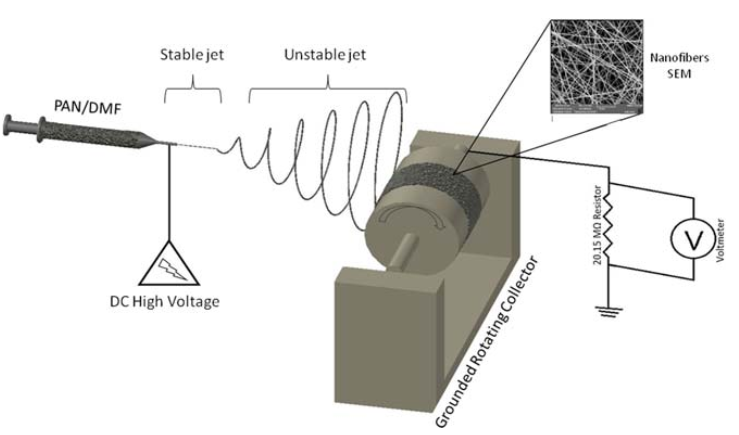
\includegraphics[width=0.75\textwidth]{./Figures/electrospinningSetup.png}
\decoRule
\caption[Far-Field Electrospinning Setup]{Schematic set-up for far-field electrospinning \cite{Nagham2017}}
\label{fig:electrospinningSetup}
\end{figure}

\section{Course Content to be Used}
For the electrosinning process purpose, a model that predicts the final fiber diameter can be used to control de electrospinning process to achieve desired fiber morphology, porosity, and physical characteristics and to improve the electrospinning efficiency \cite{Rafiei2013}. The modelling approaches in literature \cite{Feng2002, Gupta2004, Helgeson2008, Hohman2001, Reneker2006, Roozemond2007, Taylor1969, Yarin2011} divide the jet into stable and unstable regions, where different governing equations are used. The stale jet region has been modelled as an electrified jet subjected to stretching by an external $E$. The basics for modelling electrified jets were developed by Taylor \cite{Taylor1969}. The Taylor model was improved by the inclusion of the effects of jet stretching, charge transport, and $E$; this is known as the slender body model \cite{Gupta2004}. The slender body model allows the expansion of regular perturbations for long jets with integral formulations, Taylor's series expansions, weighted residuals, and variational principles \cite{Feng2002}. Feng \cite{Feng2002} derived a modified model to avoid the instability issues of the slender body model. In Feng's model, the jet is represented by four steady-state equations: the continuity equation, momentum conservation, charge conservation, and Coulomb's law. Rooxemond expanded Feng's model to account for the viscoelastic properties of the polymer solution fluid, as Feng's generalized Newtonian constitutive relations for the viscous normal stress difference.

In the stable jet region, shown in Figures \ref{fig:electrospinningSetup} and \ref{fig:electrospinningStableRegion}, the slender body approximation is assumed to model the stable viscoelastic electrospun jet, where the flow was simplified to an non-uniform elongation with all quantities depending only on the $z-axis$. The following is a interpretation of Ismail's work \cite{Ismail2016} in regards to the electrospun fibers within the stable jet region.

\begin{figure}[th]
\centering
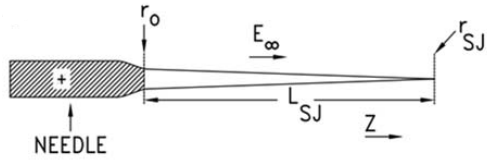
\includegraphics[width=0.75\textwidth]{./Figures/electrospinningStableRegion.png}
\decoRule
\caption[Electrospinning Stable Region]{Physical model of the electrospinning process, representing the stable jet. \cite{Ismail2016}}
\label{fig:electrospinningStableRegion}
\end{figure}

In addition, a negligible effect of solvent evaporation from the jet was assumed. Moreover, the viscoelastic Giesekus constitutive laws \cite{Hinch} were used to determine the relation between the viscous stresses in the momentum equation. The Giesekus model adds quadratic non-linearity and considers that the deviatoric stress is the sum of the solvent and polymer stresses. The current model for the stable jet region was based on Feng's model \cite{Feng2002}. With the assumptions above, the equations governing the stable jet are applicable for a specific length $L_{sj}$. $L_{sj}$ is a function of the stable model ouput parameters \cite{He2007}. He et al. He et al. \cite{He2007} provide a rational theory considering a steady-state flow of an infinite viscous jet pulled from a capillary orifice and accelerated by a constant external $E$. Since the electrical force is dominant over other forces in the stable jet, the bending instability occurs when the conductive and convective $I_{s}$ are equal. He et al. \cite{He2007} defined $L_{sj}$ as follows:

\begin{equation}
L_{\text{sj}}=\frac{4 \text{kQ}^3}{\pi \rho ^2 I^2}\left(\left(\frac{2 \varsigma_{\text{sj}}
   Q}{\text{$\pi $K$\rho $E}_{\text{sj}}}\right){}^{-\frac{2}{3}}-\frac{1}{r_0^2}\right)
\label{eq:specificLength}
\end{equation}

the mass conservation equation for the jet is as follows:

\begin{equation}
\text{$\pi $r}^2 v=Q
\label{eq:massConservation}
\end{equation}

Where $r$ and $v$ are measured at $z$. The charge conservation balance is give by Feng \cite{Feng2002}:

\begin{equation}
2 \text{$\pi $r$\varsigma$v}+\text{$\pi $r}^2 \text{kE}=I
\label{eq:chargeConservation}
\end{equation}

The forces applied on the small control volume shown in Figure \ref{fig:electrospinningForces} are the tangential and the normal components of the electric force, the viscous stress and $\gamma$. The linear momentum equation in the axial direction $z$ is given by Feng \cite{Feng2002}:

\begin{figure}[th]
\centering
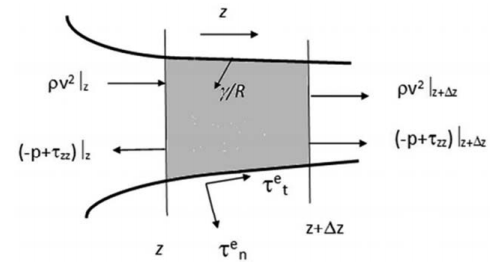
\includegraphics[width=0.75\textwidth]{./Figures/electrospinningForces.png}
\decoRule
\caption[Electrospinning Forces]{Forces applied during the electrospinning process within the stable jet. \cite{Ismail2016}}
\label{fig:electrospinningForces}
\end{figure}

\begin{equation}
\left(\tau _t^e-\frac{\tau _n^e \text{dr}}{\text{dz}}\right) 2 \pi  r+\frac{d \left(\pi  r^2
   \left(\tau _{\text{zz}}-p\right)\right)}{\text{dz}}+\frac{\gamma  \text{dr} 2 \pi  r}{r
   \text{dz}}+\rho  g \pi  r^2=\frac{d \left(\rho  \pi  r^2 v^2\right)}{\text{dz}}
\label{eq:linearMomentum}
\end{equation}

Where $\tau_{t^e}$ and $\tau_{n^e}$ are the tangential and the normal forces, respectively, per unit area exerted on the surface of the jet due to $E$. $\tau_{zz}$ is the shear stress in the axial direction $Z$, g is the gravitational acceleration, and p is the pressure. Since the sum of the normal forces at the surface of the jet is equal to zero, the following can be defined:

\begin{equation}
p+\tau _n^e=\tau _{\text{rr}}+\frac{\gamma }{r}
\label{eq:sumNormalForces}
\end{equation}

Where $\tau_{rr}$ is the shear stress in the radial direction. The Giesekus model adds quadratic non-linearity and divides the deviatoric stress into a solvent contribution and a polymer contribution \cite{Hinch} as follows:

\begin{equation}
\tau =\tau _s+\tau _p
\label{eq:shearStress}
\end{equation}

Where $\tau$ is the total shear stress, $\tau_{p}$ is the polymer shear stress, and $\tau_{s}$ is the solvent shear stress, which is deduced from the Newtonian constitutive law given by:

\begin{equation}
\tau _s=\frac{3 \eta _s \text{dv}}{\text{dz}}
\label{eq:solventShearStress}
\end{equation}

Where $\eta_{s}$ is the solution viscosity. The $\tau_{p}$ equations are obtained from the viscoelastic laws \cite{Hinch} as follows:

\begin{equation}
\tau _{\text{prr}}+\lambda  \left(v \tau _{\text{prr}}'+v' \tau
   _{\text{prr}}\right)+\frac{\alpha  \lambda  \tau _{\text{prr}}^2}{\eta _p}=-\eta _p v'
\label{eq:polymer1ShearStress}
\end{equation}

\begin{equation}
\tau _{\text{pzz}}+\lambda  \left(v \tau _{\text{pzz}}'+v' \tau
   _{\text{pzz}}\right)+\frac{\alpha  \lambda  \tau _{\text{prr}}^2}{\eta _p}=2 \eta _p v'
\label{eq:polymer2ShearStress}
\end{equation}

Where $\alpha$ is the mobility factor, $\tau_{pzz}$ and $\tau_{prr}$ are the shear stresses of the polymer in the axial and radial directions respectively, $\lambda$ is the linear charge density in $C/m$, and $\eta{_p}$ is the polymer viscosity. The prime symbol indicates the first derivative with respect to $z$.

With the substitution of equations: \ref{eq:sumNormalForces}, \ref{eq:solventShearStress}, \ref{eq:polymer1ShearStress}, and \ref{eq:polymer2ShearStress} into \ref{eq:linearMomentum}, the momentum equation in the z direction \cite{Reneker2006} becomes:

\begin{equation}
\frac{d \left(\text{$\rho $r}^2 v^2\right)}{\text{dz}}=2
   \text{r$\varsigma$E}+\frac{T_p'}{\pi }+r' \gamma +r^2
   \left(\frac{\varsigma\varsigma'}{E}-\left(\bar{\varepsilon }-\varepsilon \right)
   \text{EE}'\right)+3 \eta _s v' \text{$\pi $r}^2
\label{eq:linearMomentumExpand}
\end{equation}

Where $\varepsilon$ and $\bar{\varepsilon}$ are the permittivity of the jet and the air, respectively, $T_{p}$ is the tensile force estimated by the multiplication of the shear stresses $\left(\tau_{\text{pzz}}-\tau_{\text{prr}}\right)$ by the cross sectional area of the jet $\left(\pi r^{2}\right)$. The Equation for E was given by Reneker and Fong \cite{Reneker2006} as follows:

\begin{equation}
E\left(z\right)=E_{\infty }\left(z\right)+\ln\left(\frac{r}{L}\right) \left(\frac{I \bar{\varepsilon } (d
   \text{$\varsigma$r})}{\text{dz}}-\frac{\beta  \left(d^2 \text{Er}^2\right)}{2
   \text{dz}^2}\right)
\label{eq:Eequation}
\end{equation}

Where $\beta$ is the permittivity ratio $\left(\bar{\varepsilon } \mathbin{/} \varepsilon -1\right)$ and $L$ is the jet length. The complete derivation of the stable jet model was given in Feng's \cite{Feng2002}, and Reneker's \cite{Reneker2006} work.